Di seguito elenchiamo i principali casi d'uso per ciascun tipo di utente che interagisce col sistema. 

\paragraph{Operatore}
Una rappresentazione grafica dei casi d'uso dell'Operatore è disponibile in figura \ref{use_case_diag_operator}
\begin{figure}[h]
  \caption{Diagramma dei casi d'uso dell'Operatore}
  \label{use_case_diag_operator}
  \centering
    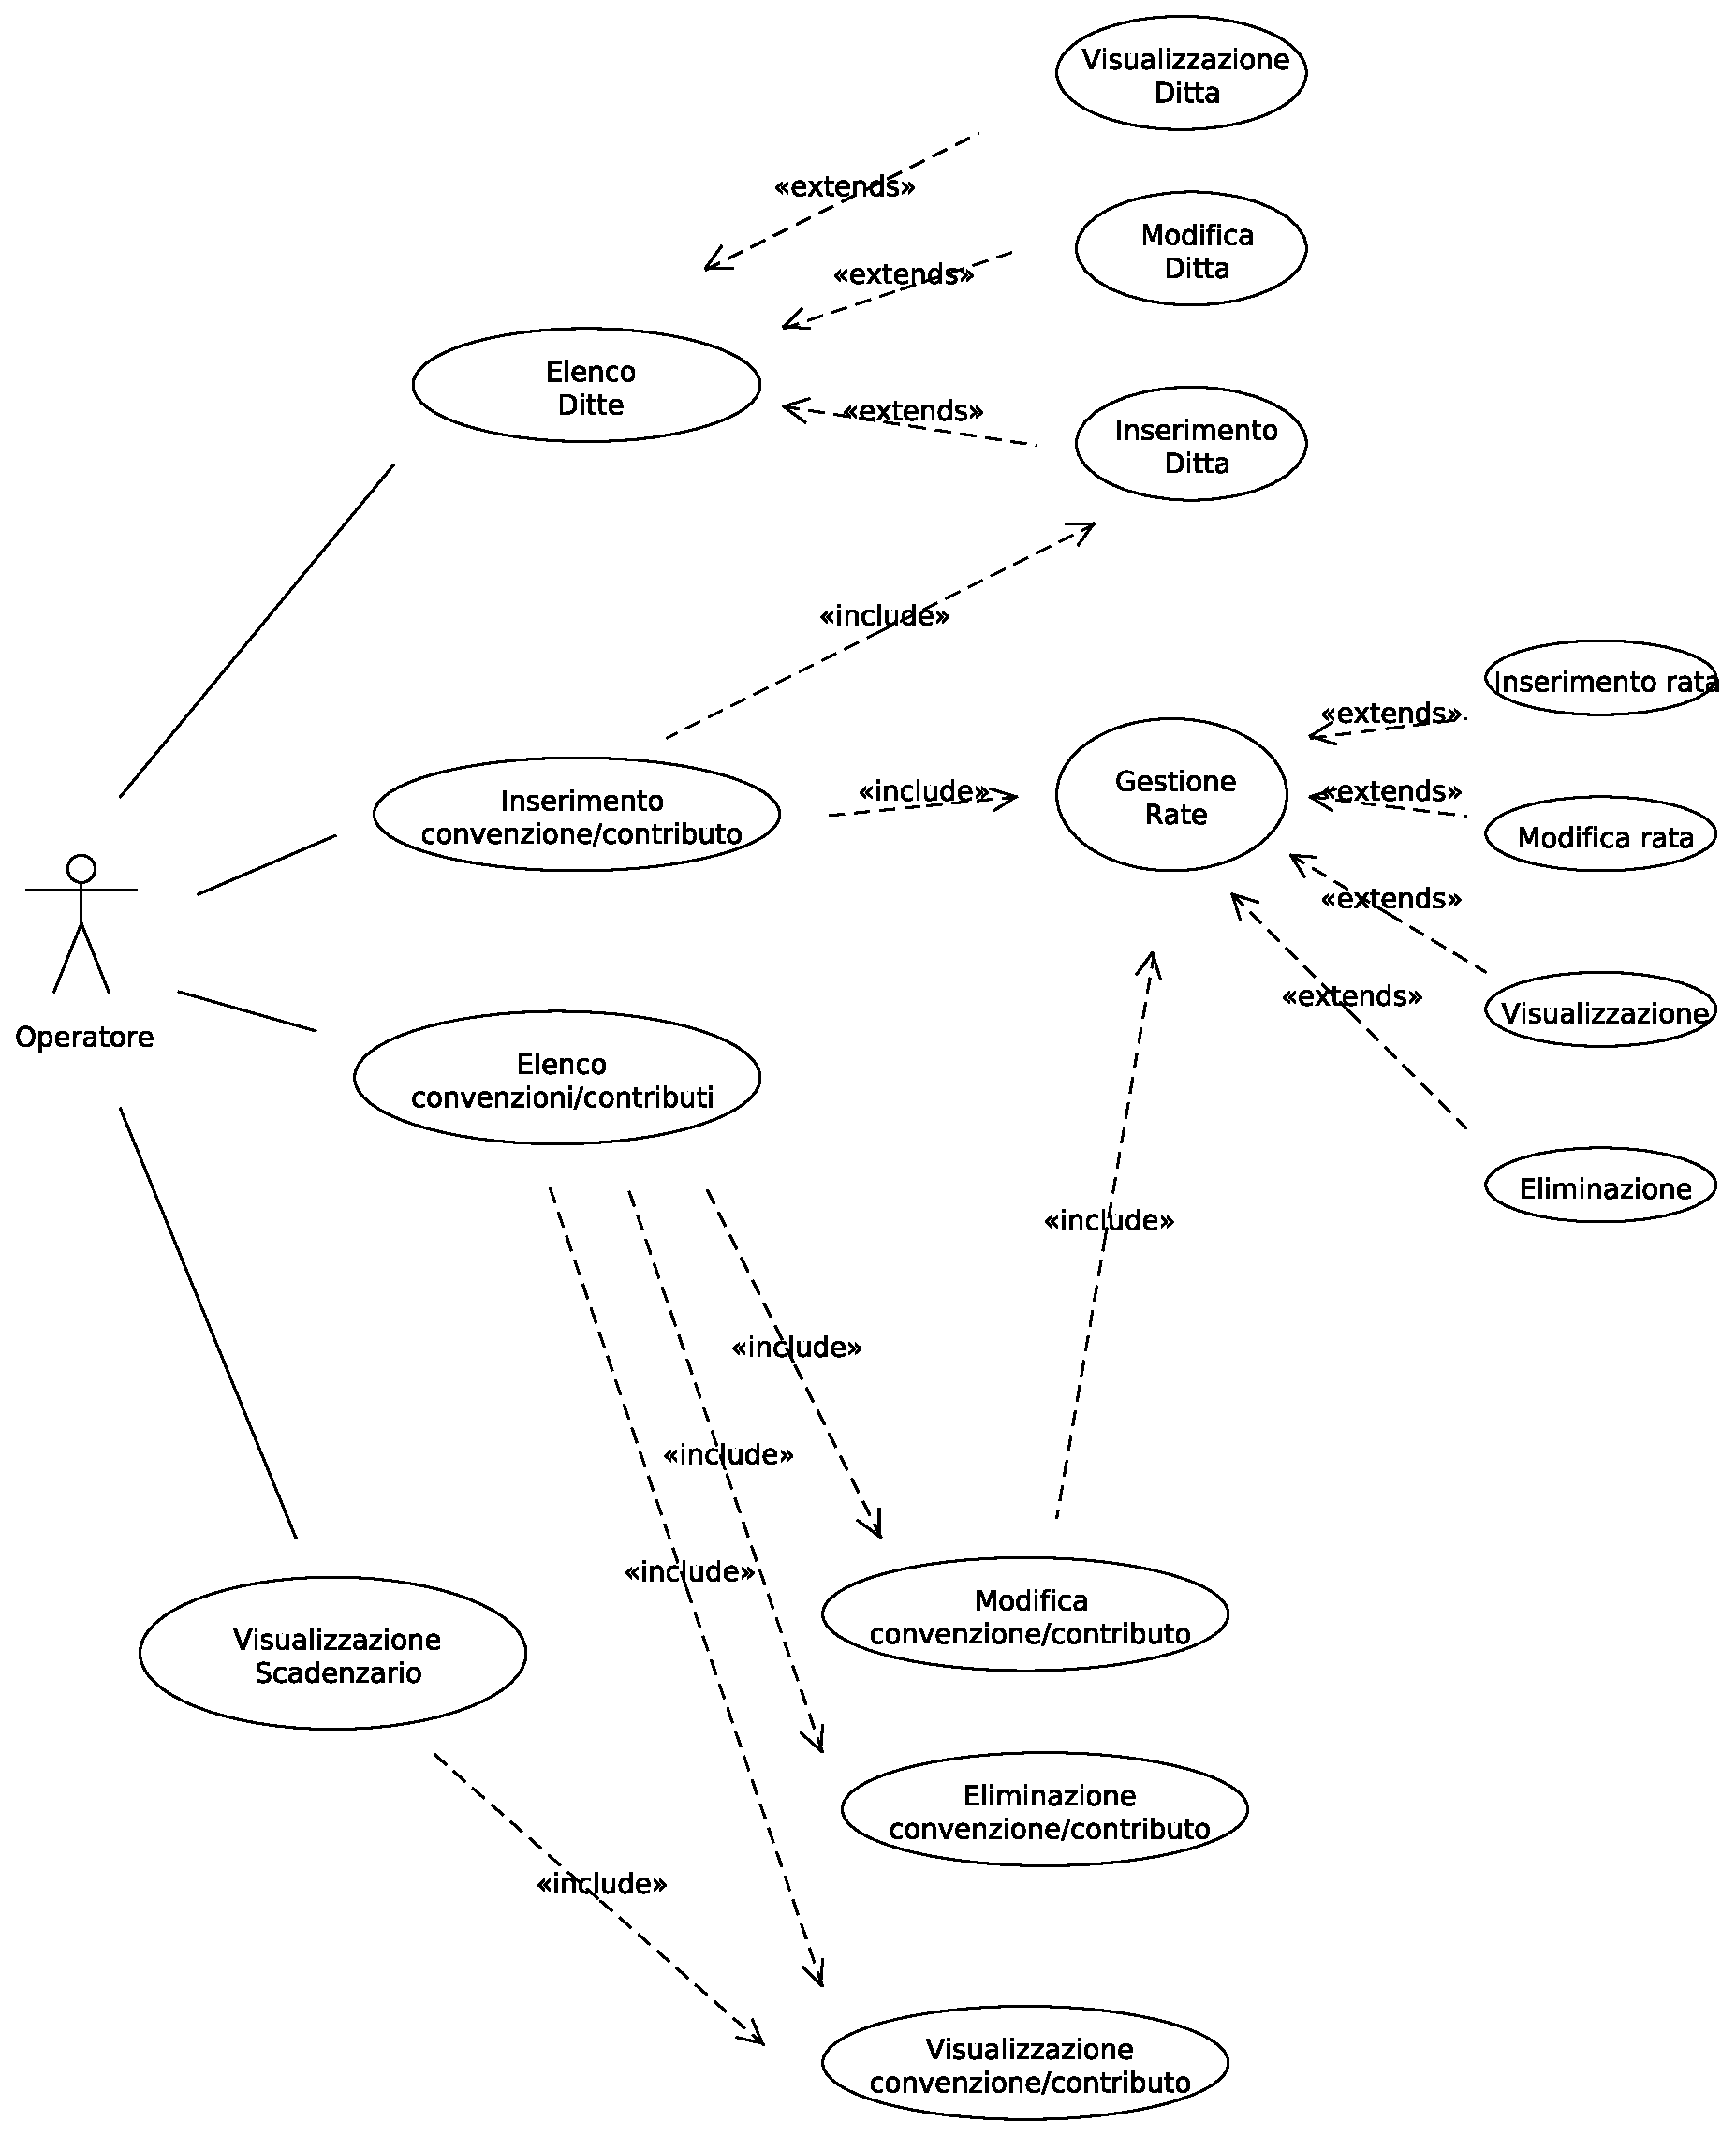
\includegraphics[width=1\textwidth]{images/casi_uso_operatore.eps}
\end{figure}

\begin{enumerate}
  \item Inserimento di una nuova Convenzione/Contributo\\
  
  Percorso base:
  l'operatore, una volta effettuato il login, clicca su ``Crea una convenzione/contributo''; viene visualizzata una schermata suddivisa in varie schede,
  ognuna corrispondente ad un passo della procedura. E' possibile passare da una vista all'altra mediante i pulsanti ``Avanti'' e ``Indietro''. I passi sono:
  \begin{enumerate}
    \item Inserimento dei dati della convenzione/contributo\\
      
      In questa scheda sono elencati tutti i campi necessari per la definizione di una convenzione/contributo, 
      che l'Operatore deve compilare. Tali campi sono:
      \begin{itemize}
	\item Il titolo
	\item Il numero di protocollo
	\item L'UAR
	\item La tipologia
	\item Il responsabile scientifico\\
	  Per selezionare un responsabile scientifico è possibile usare l'apposito menù a tendina o, in alternativa, qualora la persona cercata non sia nell'elenco, aggiungerla cliccando sul pulsante ``Aggiungi''.
	\item Il referente
	\item La dittà\\
	  Per selezionare una dittà si può usare l'apposito menù a tendina o, se la dittà cercata non fosse presente nell'elenco, aggiungerne una nuova cliccando sul pulsante ``Aggiungi''.
	\item Il nome del progetto CIA
	\item Il Repertorio
	\item Il totale imponibile
	\item L'Iva
	\item La data di approvazione
	\item La data di inizio
	\item La data di scadenza
      \end{itemize}
      
      Nota : i campi riguardanti l'Iva non sono presenti nel caso del contributo.
      
    \item Inserimento della tabella di ripartizione\\
     
      Questa scheda contiene le voci della tabella di ripartizione. L'Operatore può modificare alcuni valori percentuali 
      in base ai quali dividere l'importo totale. Le voci non modificabili sono calcolate in relazione ai campi modificabili facendo riferimento alle norme di ateneo. Le voci modificabili sono:
      \begin{itemize}
	\item Personale: stabilisce la quota destinata al personale; è l'unico campo principale che l'operatore può modificare e in base al quale vengono calcolati gli altri.
	\item Missioni, Materiale di consumo, etc. sono sottocampi di Beni e Servizi e servono per meglio specificare come verrà ripartita la quota destinata a ``Beni e Servizi''.
      \end{itemize}
    \item Gestione delle rate\\
      
      Questo passo della procedura è facoltativo: viene data la possibilità all'operatore di inserire delle rate per la convenzione/contributo
      che sta creando. Una volta inserite una o più rate
      queste vengono visualizzate in una tabella e l'Operatore
      ha la possibilità di modificare, visualizzare, eliminare una rata cliccando sui tasti ``Modifica'',``Visualizza'' ed ``Elimina'' che compaiono sulla destra, nella riga della tabella
       corrispondente alla rata in questione. Per i dettagli riquardo alle operazioni sulle rate si rimanda ai corrispettivi casi d'uso.

      
    \item Inserimento della documentazione relativa alla convenzione\\
	  
	  Questa scheda elenca i documenti allegati alla convenzione. L'Operatore può aggiungere o eliminare un documento 
	  cliccando sugli appositi tasti. Premendo il tasto ``Salva'' la convenzione viene salvata e la procedura termina. Si ritorna alla schermata precedente.
  \end{enumerate}
		 
  Percorso alternativo:
  Durante uno qualsiasi dei passi, l'Operatore può cliccare il tasto ``Annulla'', che comporta, a seguito di una conferma, il ritorno alla schermata precedente
  senza che la convenzione/contributo venga inserita o i cambiamenti effettuati salvati.
  Se l'Operatore clicca sul tasto ``Salva'' senza aver compilato dei campi obbligatori, o avendo inserito dei valori non consentiti, viene visualizzato un messaggio di errore 
  e il documento non viene salvato. La schermata non viene cambiata, in modo che l'Operatore possa procedere alla correzione.
     
  \item Visualizzazione delle convenzioni/contributi\\

  Percorso base:
  l'operatore clicca su ``Visualizza contratti''; viene mostrata una lista delle convenzioni/contributi correntemente stipulate in 
  riferimento al dipartimento di afferenza dell'Operatore, con opportuni filtri 
  per agevolare la ricerca (tra cui un filtro per data di scadenza) e ordinabili secondo la data.
  L'Operatore può selezionare una convenzione e compiere 3 azioni, per cui si rimanda ai corrispettivi casi d'uso, mediante gli appositi pulsanti, che appaiono sulla destra portando il cursore su 
  una convenzione:
  \begin{itemize}
   \item visualizzarla
   \item modificarla
   \item eliminarla
  \end{itemize}		

  Percorso alternativo:
  Si può tornare alla pagina iniziale con l'apposito tasto.
 
  \item Modifica di una convenzione\\
  
  Percorso base:
  l'Operatore a partire dalla schermata ``Visualizza Contratti'' clicca sul pulsante ``Modifica'' che appare sulla destra nella riga 
  della tabella corrispondente alla convenzione/contributo desiderata. Viene visualizzata una schermata suddivisa analoga a quella
  descritta nel caso della ``Creazione di una convenzione/contributo'' con la differenza che in questo caso è possibile spostarsi da una scheda all'altra
  cliccando sulla scheda stessa. Inoltre è presente la scheda aggiuntiva ``Riepilogo'' che contiene alcune informazioni di riepilogo come il residuo
  totale della convenzione/contributo o il totale fatturato.
  L'Operatore effettua i cambiamenti desiderati quindi clicca sul pulsante ``Salva''.\\

  Percorso alternativo:
  l'Operatore può cliccare sul tasto "Annulla" in qualsiasi momento per tornare alla schermata "Visualizzazione delle convenzioni" senza salvare le modifiche effettuate.
  Se l'Operatore clicca su "Salva" ma alcuni valori immessi non sono corretti, viene visualizzato un messaggio di errore e non si torna alla schermata "Visualizzazione delle
  convenzioni". I cambiamenti effettuati non vengono (ovviamente) salvati.
  
\item Visualizzazione di una convenzione/contributo\\
 
  Del tutto analogo a ``Modifica di una convenzione/contributo'' con la differenza che in questo caso non è possibile modificare i dati della
  convenzione/contributo.
  
  
  
\item Inserimento di una rata\\
Percorso base:
l'operatore può inserire una rata sia in fase di creazione della convenzione/contributo sia in fase di modifica; in entrambi i casi dopo aver raggiunto
la scheda ``Rate'' l'Operatore clicca sul pulsante ``Aggiungi una rata''.  
Viene visualizzata una finestra di dialogo suddivisa in varie schede,
ognuna corrispondente ad un passo della procedura. E' possibile passare da una scheda all'altra mediante i pulsanti "Avanti" e "Indietro". I passi sono:
\begin{enumerate}
  \item Inserimento dei dati della rata\\
  
  L'operatore inserisce i seguenti campi
    \begin{itemize}
    \item Importo
    \item Iva
    \item Data
    \item Numero Reversale
    \item Data Reversale
    \item Numero di Sospeso
    \item Numero di fatturato
    \item Data fatturata
    \item E'stata pagata la fattura?
    \item Deve essere allegata la fattura?
    \item Note
    \end{itemize}
    
   Nota : i campi riguardanti l'Iva non sono presenti nel caso del contributo.

   
  \item Inserimento della tabella di ripartizione\\
  
  Il procedimento è del tutto analogo  a quello descritto nel caso d'uso "Inserimento della tabella di ripartizione" per l'inserimento di 
  una nuova convenzione/contributo. 
\end{enumerate}

Le modifiche vengono salvate cliccando sul pulsante "Salva". Si ritorna alla schermata precedente;

Percorso alternativo:
l'Operatore clicca sul pulsante ``Annulla'', viene chiusa la finestra di dialogo senza che la rata sia stata inserita.

\item Modifica di una rata\\

Percorso base:
l'Operatore accede alla schermata ``Visualizza contratti'' cliccando sul pulsante apposito nella pagina iniziale, quindi seleziona la convenzione/contributo alla quale la rata appartiene e clicca sul pulsante ``Modifica'' che compare
all'interno della riga selezionata. Viene così visualizzata la schermata ``Modifica di una convenzione/contributo''; l'Operatore raggiunge la scheda ``rate'' e clicca sul pulsante ``Modifica'' che compare selezionando la riga della tabella
corrispondente alla rata desiderata. Viene visualizzata una finestra di dialogo composta di varie schede analoghe a quelle descritte nel caso dell'inserimento. E' possibile passare da una scheda all'altra cliccando su di esse.
Dopo avere effettuato le modifiche richieste l'Operatore clicca sul pulsante ``Salva'', la convenzione/contributo viene aggiornata e viene visualizzata la schermata precedente.

Percorso alternativo:
l'Operatore clicca sul pulsante ``Annulla'', le modifiche vengono scartate e si torna alla schermata precedente.

\item Visualizzazione di una rata

Una volta raggiunta la scheda ``rate'' relativa alla convenzione/contributo di interesse l'Operatore, dopo aver selezionato la rata desiderata, clicca sul pulsante ``Visualizza''. Viene presentata una finestra di dialogo analoga a quella descritta nel caso della modifica 
con la differenza che i campi non sono modificabili. E' possibile tornare alla schermata precedente cliccando sul pulsante ``Indietro''.

\item Eliminazione di una rata\\

Una volta raggiunta la scheda ``rate'' relativa alla convenzione/contributo di interesse l'Operatore, dopo aver selezionato la rata di interesse, clicca sul pulsante ``Elimina'; appare una finestra di dialogo che chiede di confermare
l'eliminazione, l'Operatore clicca ''Sì'', la rata viene eliminata.



\end{enumerate}

 
\paragraph{Docente}
I casi d'uso del Docente sono rappresentati in figura \ref{use_case_diag_teacher}
\begin{figure}[h]
  \caption{Diagramma dei casi d'uso del Docente}
  \label{use_case_diag_teacher}
  \centering
    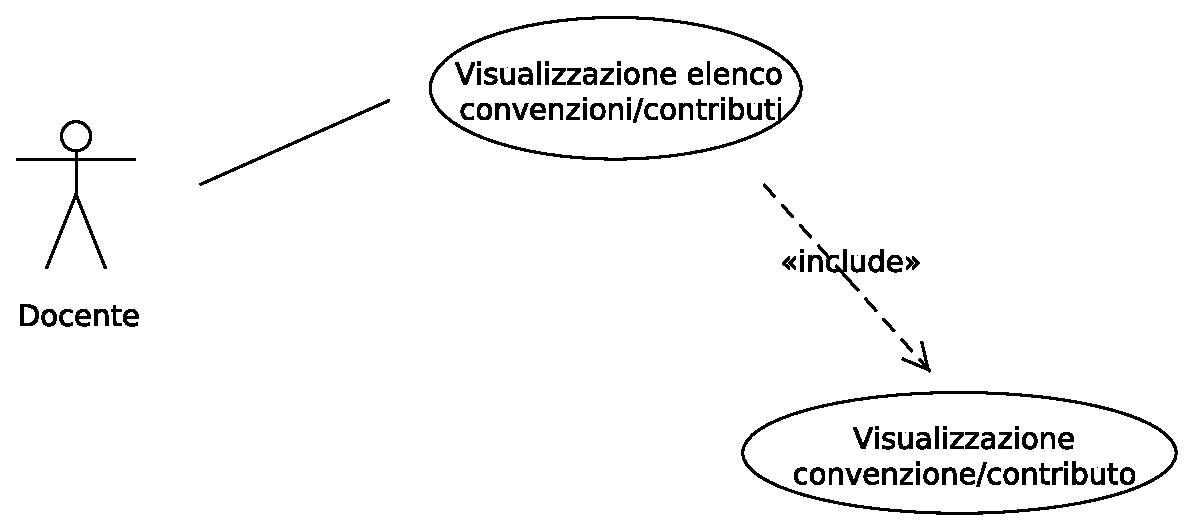
\includegraphics[width=0.8\textwidth]{images/casi_uso_docente.eps}
\end{figure}

\begin{enumerate}
 
 \item Visualizzazione dell'elenco delle convenzioni/contributi\\
 
 Il docente, dopo aver effettuato il login, può cliccare sul pulsante ``Visualizzazione della lista delle convenzioni/contributi''; la schermata
 che viene visualizzata contiene una tabella che elenca le convenzioni/contributi del docente. E' possibile filtrare le convenzioni/contributi
 secondo vari criteri(data, tipo, scadenze più vicine, ...).Inoltre è possibile visualizzare i dettagli di una convenzione/contributo cliccando sul
 pulsante ``Visualizza'' che appare posizionando il puntatore su una riga della tabella.
 
 \item Visualizzazione di una convenzione/contributo di cui il docente è responsabile scientifico\\
 
 Il docente dalla schermata ``Lista delle convenzioni/contributi'' può cliccare sul pulsante ``Visualizza'' relativo ad una convenzione/contributo; compare una schermata suddivisa in schede analoga a quella della modifica/creazione
 della convenzione. Il docente può navigare fra le schede cliccandoci sopra. Non è permessa nessuna modifica ai dati della convenzione/contributo tuttavia il docente può inserire degli allegati dalla scheda ``Allegati''. Cliccando su ``Salva''
 gli allegati inseriti dal docente vengono memorizzati, al contrario cliccando su ``Indietro'' le modifiche vegono scartate.
 
 
 
\end{enumerate}



\paragraph{Amministratore}
\begin{enumerate}
 \item Inserimento di un nuovo utente
 \item Visualizzazione della lista degli utenti
\end{enumerate}

\paragraph{Tempo}
I casi d'uso del Tempo sono rappresentati in figura \ref{use_case_diag_teacher}
\begin{figure}[h]
  \caption{Diagramma dei casi d'uso del Tempo}
  \label{use_case_diag_time}
  \centering
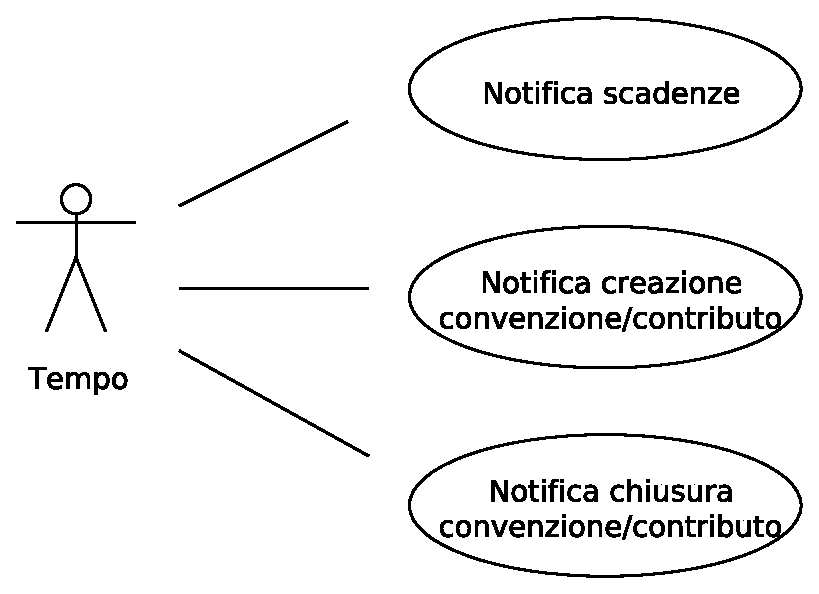
\includegraphics[width = 0.5\textwidth]{images/casi_uso_tempo.eps}
\end{figure}
\begin{enumerate}
 \item Notifica delle scadenze\\
 
    Ad intervalli periodici stabiliti, i docenti che hanno convenzioni/contributi attive con rate in scadenza ravvicinata, vengono avvertiti tramite posta elettronica.
  
 
 \item Notifica della creazione di una nuova convenzione/contributo\\
 
    Al momento del completamento della creazione di una nuova convenzione/contributo viene inviata una email all'indirizzo di posta elettronico del responsabile scientifico indicato per la convenzione/contributo. Tale email contiene
    le informazioni principali che caratterizzano la convenzione/contributo.
  
  
 \item Notifica della chiusura di una convenzione/contributo\\
 
    Al momento della chiusura di una convenzione/contributo (ovvero quando il fatturato è pari all'importo totale) viene inviata una email all'indirizzo di posta elettronico del responsabile scientifico che notifica la chiusura della
    convenzione/contributo riportando alcuni dati di questa.
\end{enumerate}




